	\chapter{Ο πηρύνας της Μηχανής}
	
	Όταν ένα framework επεκτείνεται και διακλαδώνεται και σε πολλές υπο-βιβλιοθήκες, στηρίζεται στη θεμελιώση ενός framework core, του πηρύνα της βιβλιοθήκης, στον οποίο βασίζονται οι διάφορες επεκτάσεις και υλοποιήσεις. Το \gls{API} του πηρύνα πρέπει να αποτελείται από αφαιρέσεις, οι οποίες εκθέτουν μόνο τα απολύτος απαραίτητα, ώστε οι υποβιβλιοθήκες που χρησιμοποιούν τον πηρύνα να μην δεσμεύονται σε υλοποιήσεις και να περιορίζονται σε συγκεκριμένο pipeline χρήσης για αποφυγή απρόβλεπτων συμπεριφορών. \cite{jaroslav08}
	
	\begin{theorem}[First test theorem]
		This is a test theorem.
	\end{theorem}

	\section{Game Loop}
	\begin{figure}
		\centering
		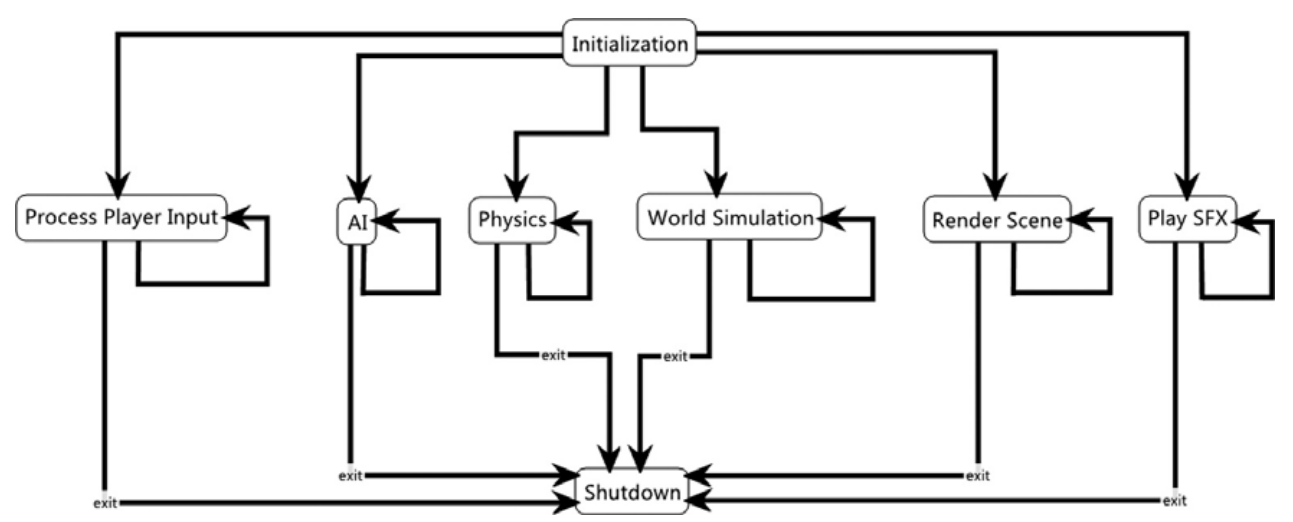
\includegraphics[width=160mm]{Images/game_coding_complete_chapter7_gameloops}
		\caption{game loops}
		\label{fig:gameloops}
	\end{figure}
		
	\section{ScreenSystem}
	\begin{figure}
		\centering
		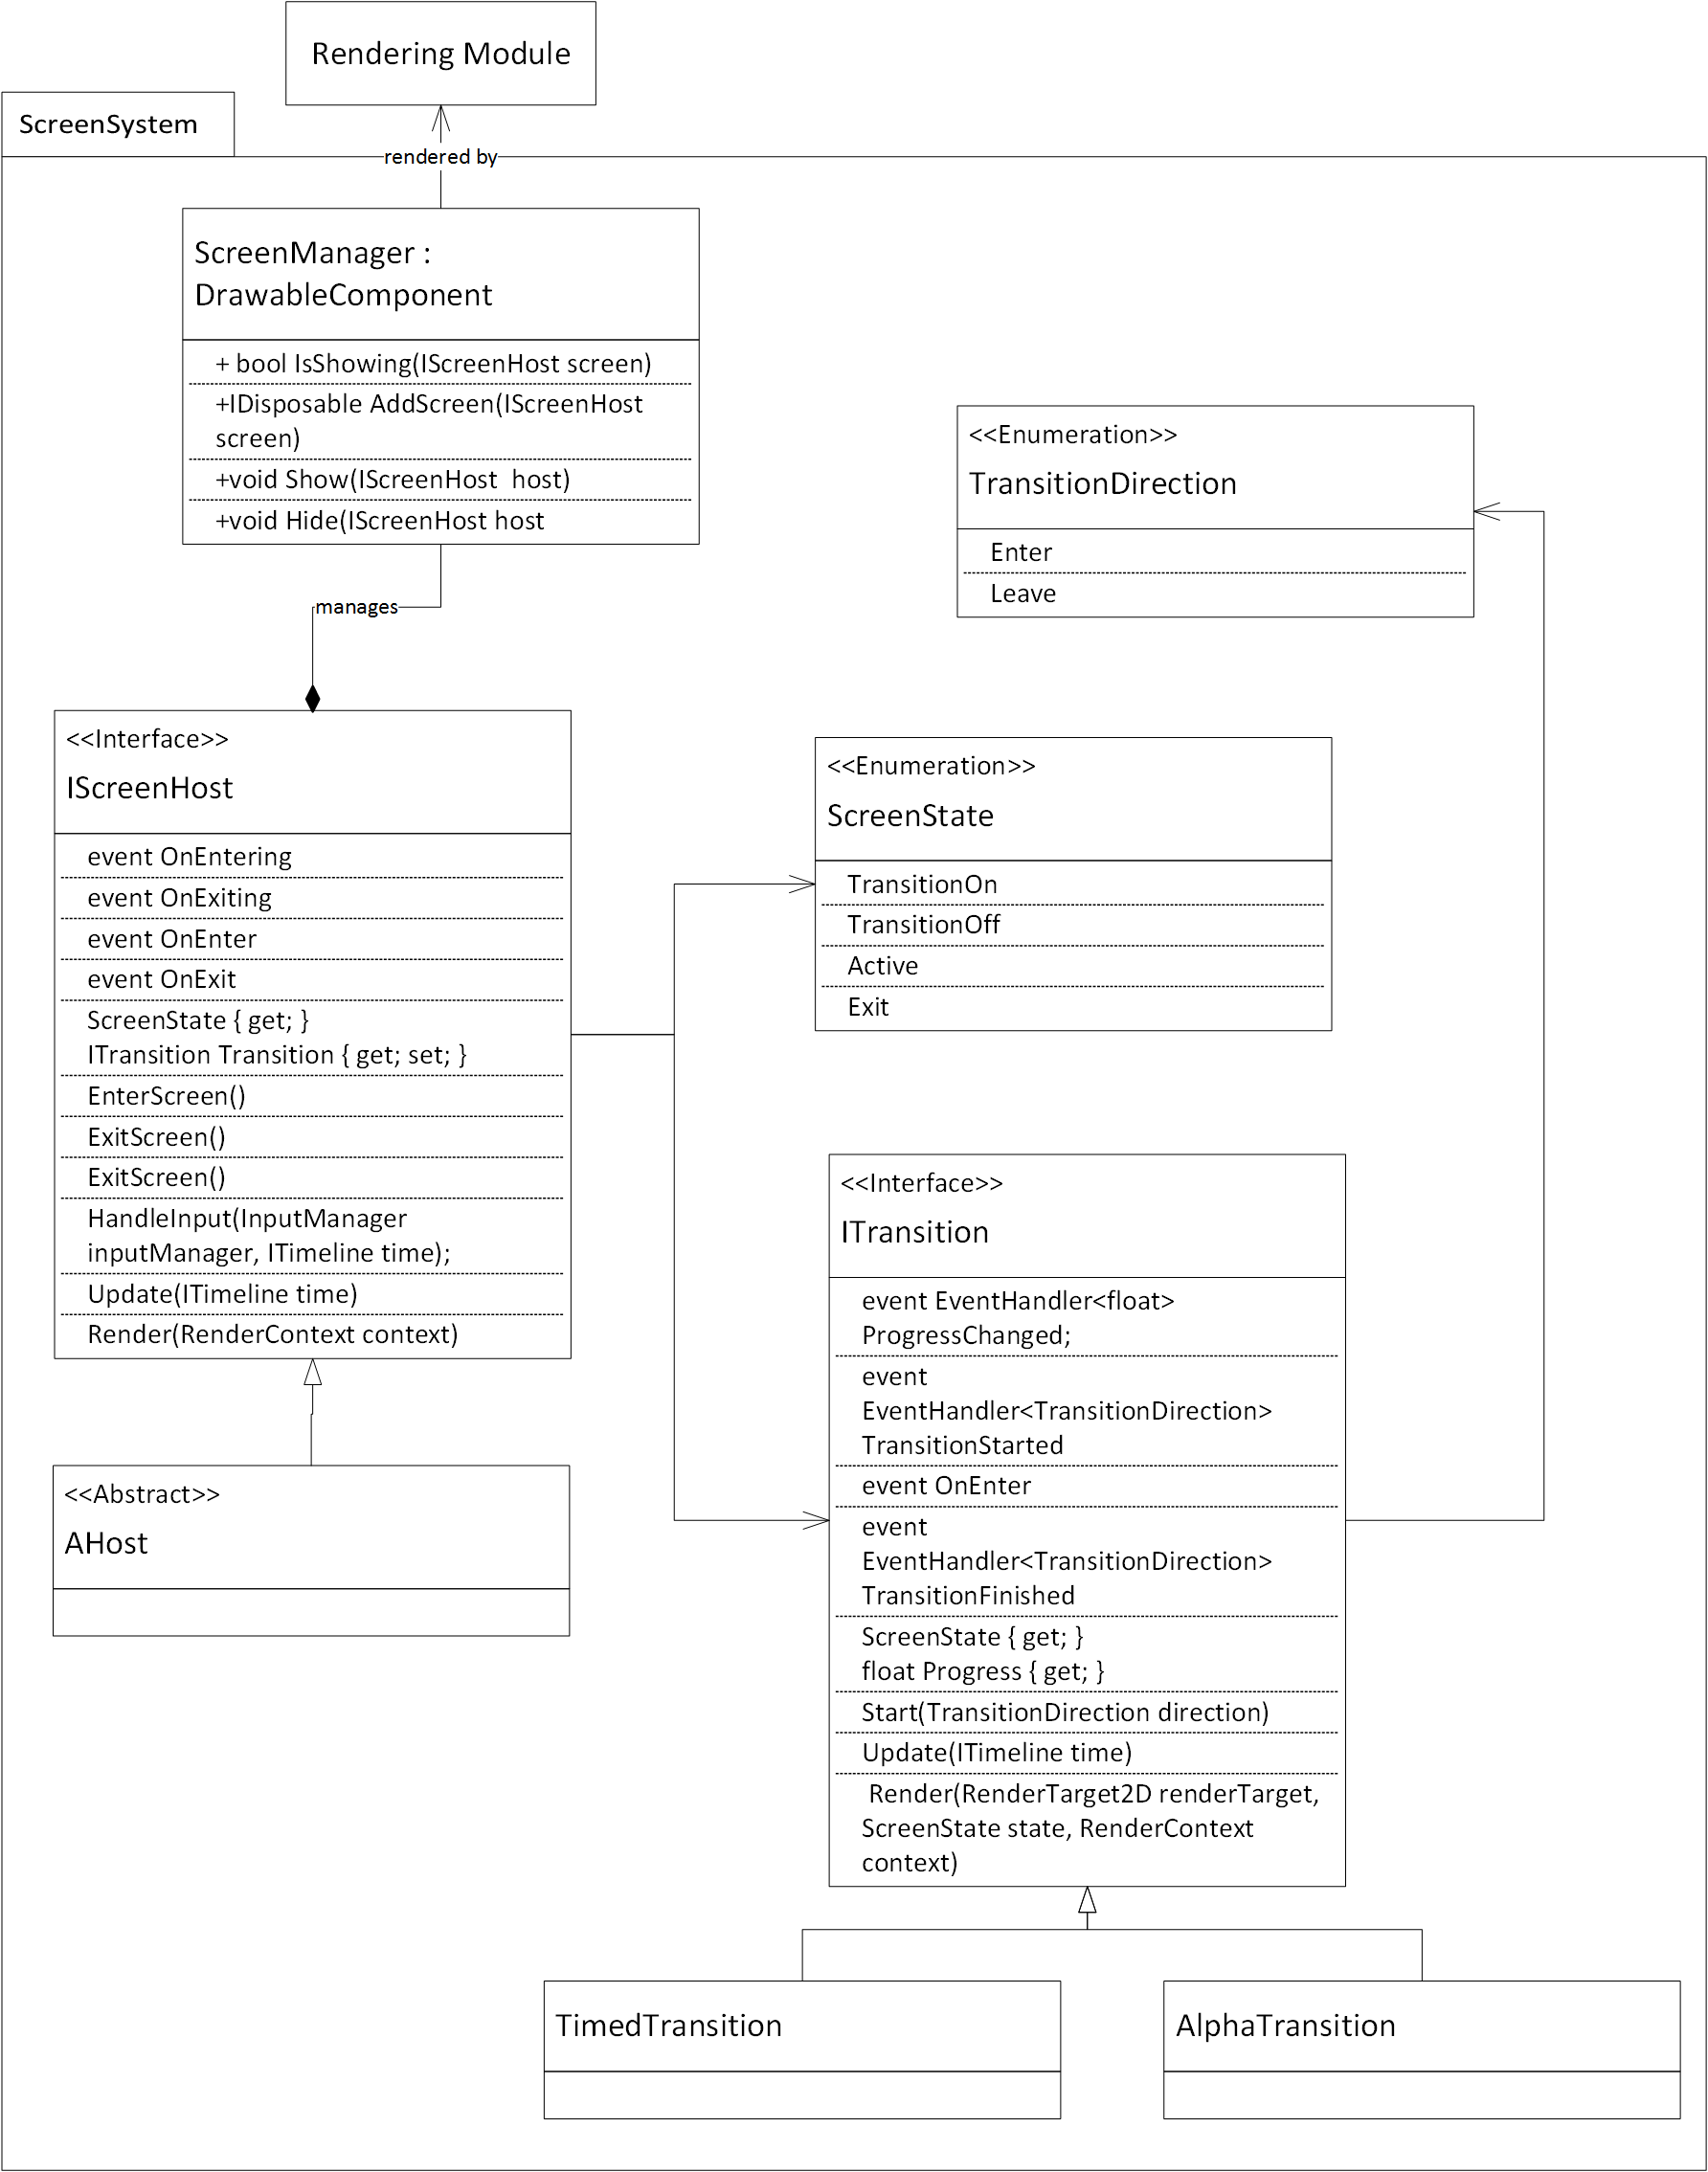
\includegraphics[width=160mm]{Images/core_screensystem}
		\caption{core screensystem}
		\label{fig:core_screensystem}
	\end{figure}	
	
	\section{Input System}
	\begin{figure}
		\centering
		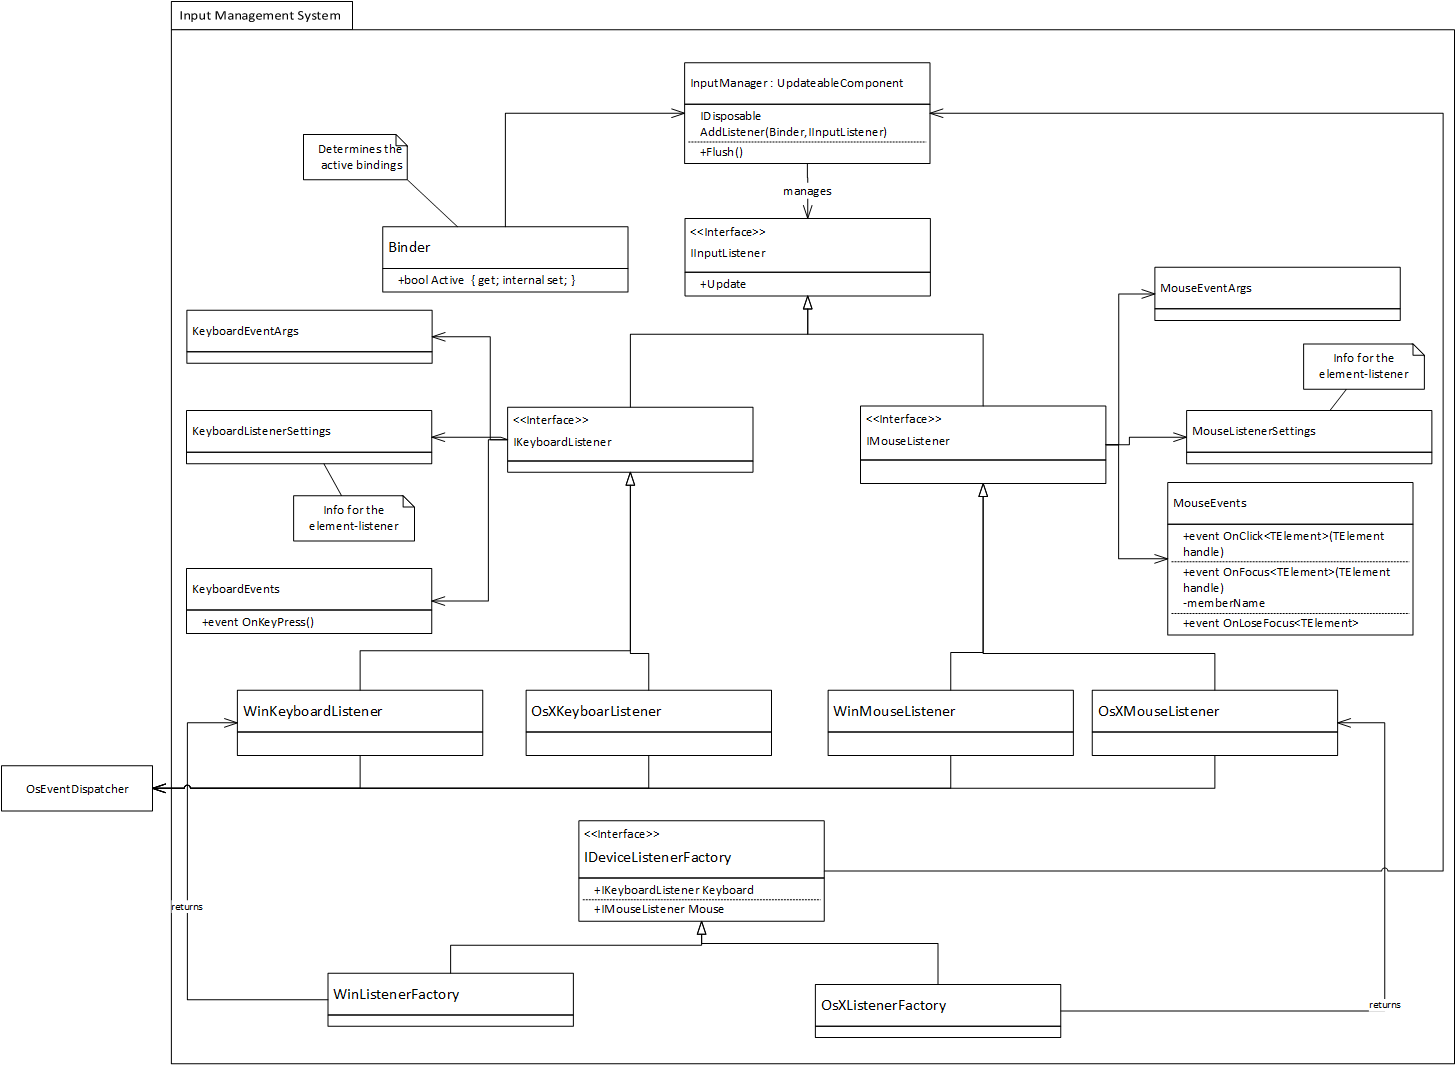
\includegraphics[width=160mm]{Images/core_input}
		\caption{core input}
		\label{fig:core_input}
	\end{figure}	